\subsubsection{Estrutura}

% SLIDE DE ESTRUTURA
\begin{frame}
\frametitle{Estrutura}

\begin{columns}
        \column{0.5\textwidth}
        \begin{figure}
            \centering
            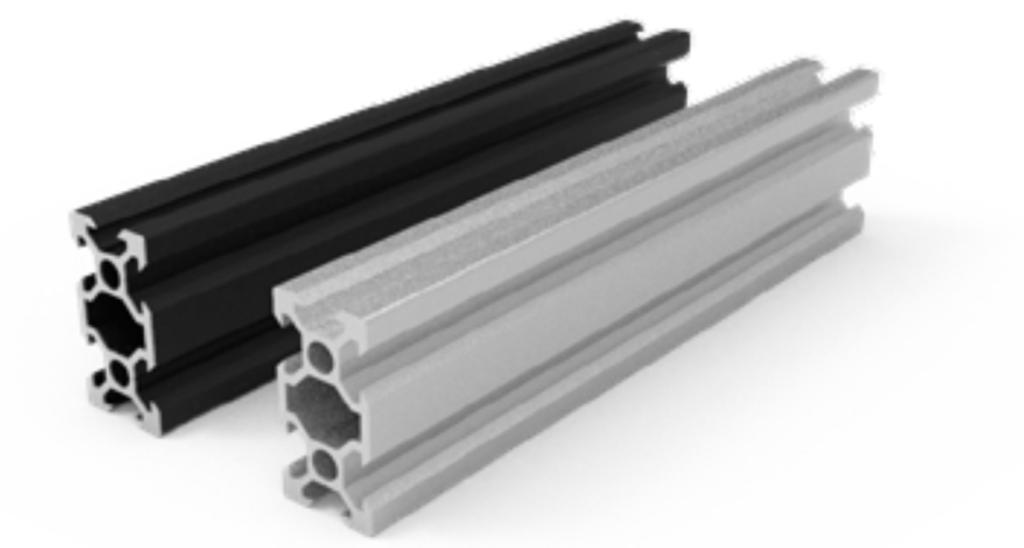
\includegraphics[scale = 0.14]{figuras/p20x40p}
            \caption{Perfil V-slot  20~x~40~mm em alumínio.}
        \end{figure}
        \column{0.5\textwidth}
        \begin{figure}
            \centering
            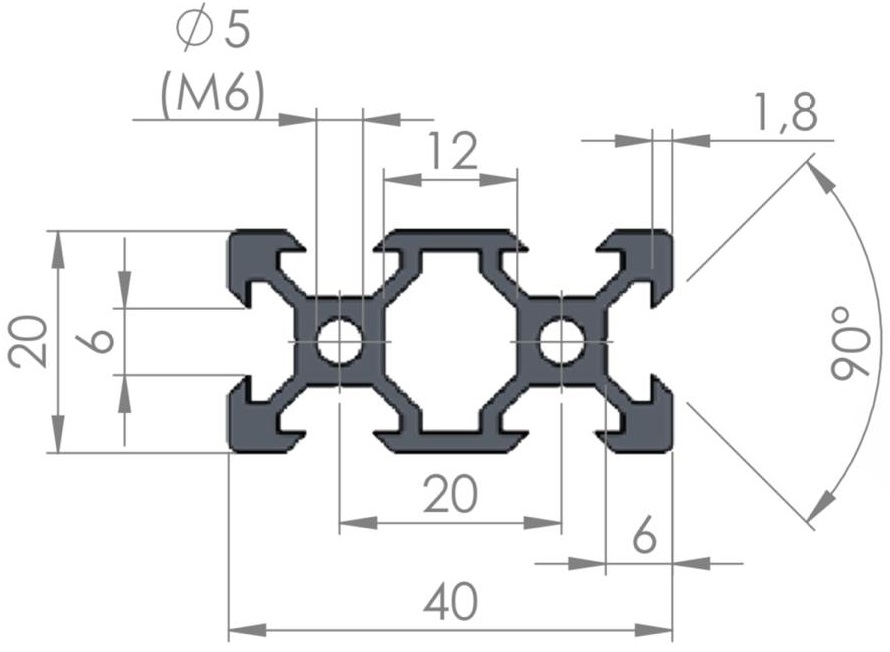
\includegraphics[scale = 0.14]{figuras/p20x40d.jpeg}
            \caption{Dimensões do perfil 20~x~40~mm.}
        \end{figure}
\end{columns}

\end{frame}

% SLIDE DE ESTRUTURA
\begin{frame}
    \frametitle{Estrutura}
    
    \begin{figure}
    \centering
    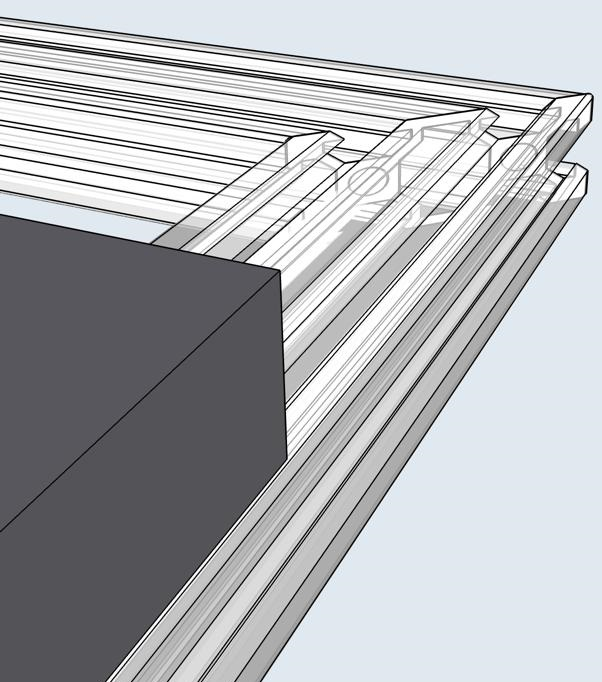
\includegraphics[scale = 0.30]{figuras/detalhe45}
    \end{figure}  
        
    \end{frame}
    
    % SLIDE DE ESTRUTURA
    \begin{frame}
    \frametitle{Estrutura}
    
    \begin{columns}
        \column{0.5\textwidth}
        \begin{figure}
            \centering
            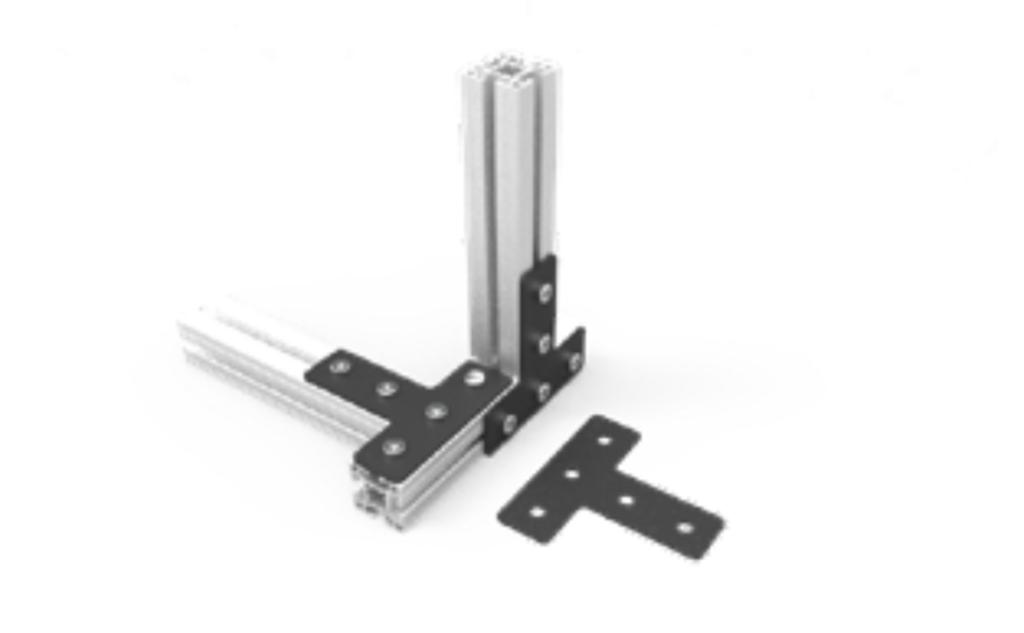
\includegraphics[scale = 0.14]{figuras/placatp}
            \caption{Placa T simples de aço.}
        \end{figure}            
        \column{0.5\textwidth}
        \begin{figure}
            \centering
            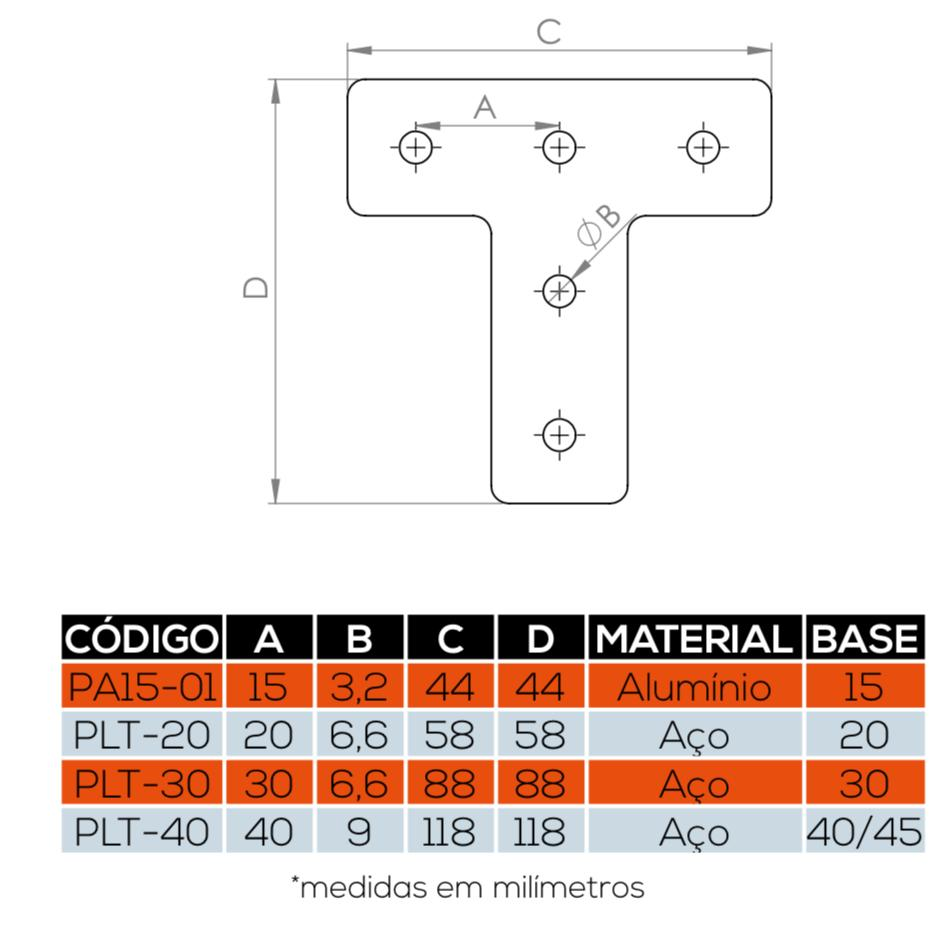
\includegraphics[scale = 0.12]{figuras/placatd}
            \caption{Dimensões da placa T simples.}
        \end{figure}            
    \end{columns}        
\end{frame}
    
% SLIDE DE ESTRUTURA
\begin{frame}
\frametitle{Estrutura}
\begin{columns}
    \column{0.5\textwidth}
    \begin{figure}
        \centering
        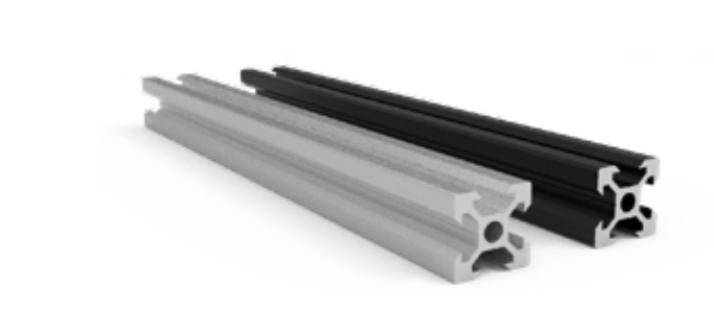
\includegraphics[scale = 0.20]{figuras/p20x20p}
        \caption{Perfil V-Slot 20~x~20~mm em alumínio.}
    \end{figure}    
    \column{0.5\textwidth}
    \begin{figure}
        \centering
        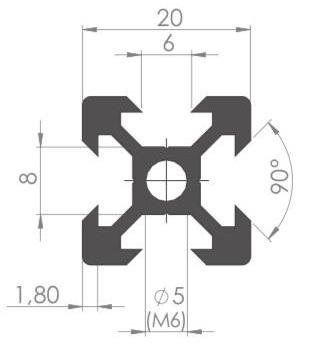
\includegraphics[scale = 0.20]{figuras/p20x20d}
        \caption{Dimensões do perfil 20~x~20~mm.}
    \end{figure}    
\end{columns}    
\end{frame}

% SLIDE DE ESTRUTURA
\begin{frame}
\frametitle{Estrutura}
\begin{columns}
    \column{0.5\textwidth}
    \begin{figure}
        \centering
        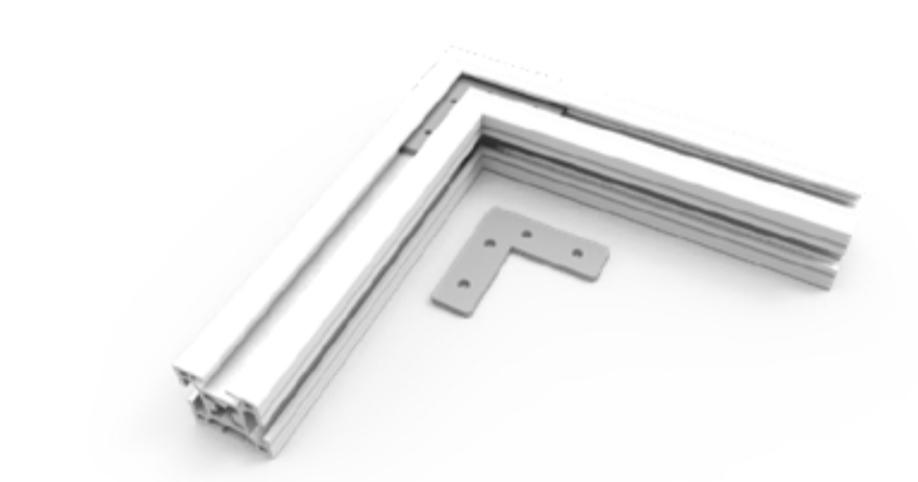
\includegraphics[scale = 0.15]{figuras/pconexao90p}
        \caption{Placa de conexão interna de 90°.}
    \end{figure}        
    \column{0.5\textwidth}
    \begin{figure}
        \centering
        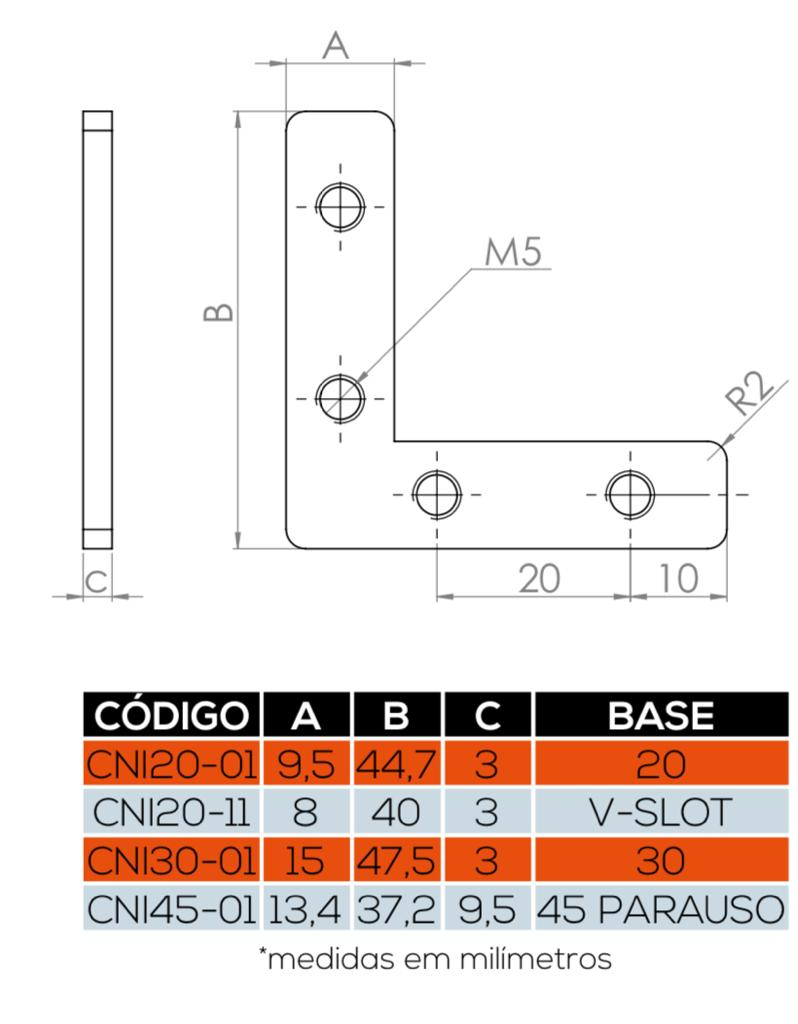
\includegraphics[scale = 0.10]{figuras/pconexao90d}
        \caption{Dimensões da placa de conexão interna de 90°.}
    \end{figure}        
\end{columns}    
\end{frame}

% SLIDE DE ESTRUTURA
\begin{frame}
\frametitle{Estrutura}

\begin{figure}
\centering
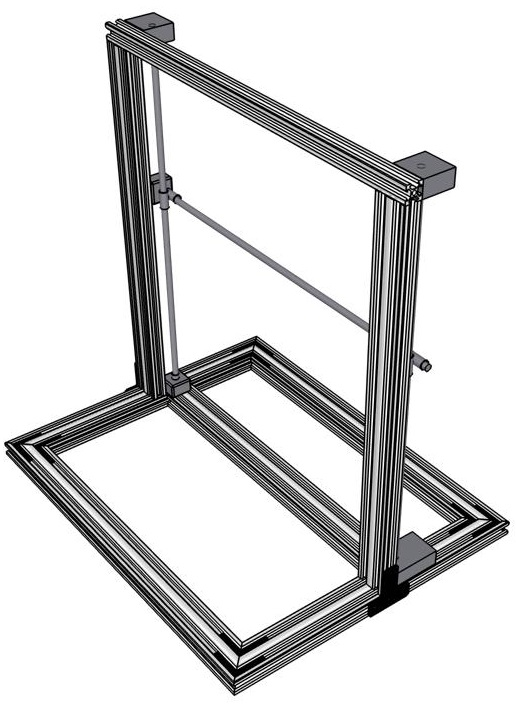
\includegraphics[scale = 0.30]{figuras/estruturamesa}
\end{figure}  

\end{frame}
    
